% !TEX TS-program = pdflatex
% !TEX encoding = UTF-8 Unicode

% This is a simple template for a LaTeX document using the "article" class.
% See "book", "report", "letter" for other types of document.

% Schriftgröße
% Schrifttype: Bei der Seitenzahlvorgaben wird eine gängige  12-Punkt-Schrift (z.B. 
% Arial oder Times New Roman) zugrunde gelegt.
\documentclass[fontsize=12pt,parskip=false,numbers=enddot]{scrartcl} % use larger type; default would be 10pt

% no indent, no parskip
\setlength{\parindent}{0pt}

\usepackage[utf8]{inputenc} % set input encoding (not needed with XeLaTeX)
\usepackage{ngerman}
\usepackage[ngerman]{babel}
\usepackage[T1]{fontenc}
\pagestyle{plain}

%\usepackage[scaled]{helvet}
\usepackage{times}	%Times New Roman font
%\usepackage{pslatex}
%\renewcommand{\baselinestretch}{1.5}

%%%%%%%%%%%%%%%%%%%%%%%%%%%
% URLs
% 
\usepackage{url}
\urlstyle{same}
% we could also use hyperref...

%%%%%%%%%%%%%%%%%%%%%%%%%%%
%
% PAGE DIMENSIONS
%
% Randbreite: Auf der linken Seite des Blattes ist ein Rand von etwa 6 cm Breite freizu-
% lassen, auf der rechten Seite ein solcher von 1,5 cm. Am oberen Seitenrand sind 3 cm 
% freizuhalten (in diesem Bereich steht die Seitenzahl), am unteren Blattende 2,5 cm.
\usepackage{geometry} % to change the page dimensions
\geometry{a4paper} % or letterpaper (US) or a5paper or....
\geometry{left=6cm}
\geometry{right=1.5cm}
\geometry{top=3cm}
\geometry{bottom=2.5cm}

% Für Grafiken
% \includegraphics[!tb][widht=10cm]{}
\usepackage{graphicx} % support the \includegraphics command and options


%\usepackage[parfill]{parskip} % Activate to begin paragraphs with an empty line rather than an indent
%\usepackage{parskip}
%\normalbaselines


%%% PACKAGES
\usepackage{booktabs} % for much better looking tables
\usepackage{array} % for better arrays (eg matrices) in maths
\usepackage{paralist} % very flexible & customisable lists (eg. enumerate/itemize, etc.)
\usepackage{verbatim} % adds environment for commenting out blocks of text & for better verbatim
\usepackage{subfig} % make it possible to include more than one captioned figure/table in a single float
% These packages are all incorporated in the memoir class to one degree or another...

%%% HEADERS & FOOTERS
\usepackage{fancyhdr} % This should be set AFTER setting up the page geometry
\pagestyle{fancy} % options: empty , plain , fancy
\renewcommand{\headrulewidth}{0pt} % customise the layout...
\lhead{}\chead{}\rhead{\thepage}
\lfoot{}\cfoot{}\rfoot{}

%%%%%%%%%%%%%%%%%%%%%%%%%%%%%
%
% SECTION TITLE APPEARANCE
%
% For indention of the subsection and subsubsection commands and overall styl factors for baselineskip
%
\RedeclareSectionCommand[
  beforeskip=-.5\baselineskip,
  afterskip=.25\baselineskip]{section}
\RedeclareSectionCommand[
  beforeskip=-.5\baselineskip,
  afterskip=0.01\baselineskip,
indent=1em]{subsection}
\RedeclareSectionCommand[
  beforeskip=-.5\baselineskip,
  afterskip=.25\baselineskip,
indent=2.5em]{subsubsection}
%\usepackage{sectsty}
%\allsectionsfont{\sffamily\mdseries\upshape} % (See the fntguide.pdf for font help)
%\allsectionsfont{\rmfamily\bfseries\normalsize}

%add a dot after the section number 
%\makeatletter
%\def\@seccntformat#1{\csname the#1\endcsname.\quad}
%\makeatother

%\usepackage{etoolbox}
\setkomafont{section}{\normalfont\bfseries}
\setkomafont{subsection}{\normalfont\bfseries}
\setkomafont{subsubsection}{\normalfont\bfseries}
%\makeatletter
%\patchcmd{\@maketitle}{\titlefont\huge}{\titlefont\small}{}{}
%\makeatother


%%% ToC (table of contents) APPEARANCE
\usepackage[nottoc,notlof,notlot]{tocbibind} % Put the bibliography in the ToC
\usepackage[titles,subfigure]{tocloft} % Alter the style of the Table of Contents
\renewcommand{\cftsecfont}{\rmfamily\mdseries\upshape}
\renewcommand{\cftsecpagefont}{\rmfamily\mdseries\upshape} % No bold!

%Add a dot after the section number in TOC.
\renewcommand{\cftsecaftersnum}{.}
\renewcommand{\cftfigaftersnum}{.}
\renewcommand{\cfttabaftersnum}{.}
\renewcommand{\cftsubsecaftersnum}{.}
\renewcommand{\cftsubsubsecaftersnum}{.}


%\renewcaptionname{ngerman}{\contentsname}{Inhalt}
%\renewcaptionname{ngerman}{\listfigurename}{Abbildungen}
%\renewcaptionname{ngerman}{\listtablename}{Tabellen}
\renewcaptionname{ngerman}{\figurename}{Abb.}
\renewcaptionname{ngerman}{\tablename}{Tab.}

%%%%%%%%%%%%%%%%%%%%%%%%%%%%%%%%%%%%%%%%%%%%%%%%%%%%%%%%%%%%
% Define some Keywords
\newcommand{\TitleGer}{Titel der Master-Thesis}	%Titel der Thesis
\newcommand{\myDegree}{Master-Thesis}		%Master-Thesis / Bachelor-Thesis
\newcommand{\myName}{Vorname Nachname}	%eigener Name
\newcommand{\myProf}{Prof.~Dr.~M.~Göcke}	%Professor
\newcommand{\myPlace}{DeinOrt}	                     %Ort
\newcommand{\myStreet}{Deine Str.~7}                   %Straße
\newcommand{\myTime}{30.05.2016} 	                     %Ausgabedatum
\newcommand{\myDate}{30.11.2016}	                     %Abgabedatum



%%%%%%%%%%%%%%%%%%%%%%%%%%%%%%%%%%%%%%%%%%%%%
% 
% Define Abbreviations
\usepackage{xspace}
\newcommand{\zb}{z.\,B.\xspace}
\newcommand{\vgl}{vgl.\xspace}
\newcommand{\Vgl}{Vgl.\xspace}
%\newcommand{\dh}{d.\,h.\xspace}


\usepackage{setspace}
\linespread{1.53}


\newcommand{\bib}[5]{\textbf{#1} \normalfont({#2}), {#3}, \url{#4}, {#5}.

}

%%%%%%%%%%%%%%%%%%%%%%%%%%%%%%%%%%%%%%%%%%%%%%%%%%%%%%%%%%%
%
% LaTeX Layout for Master Thesis @ University Giessen, Prof. Göcke.
% 
% Title is generated in "titel.tex"
%
% Designed by Robert Eber
%
%
%
%
%%%%%%%%%%%%%%%%%%%%%%%%%%%%%%%%%%%%%%%%%%%%%%%%%%%%%%%%%%%

\usepackage{lipsum}	

\begin{document}
\thispagestyle{empty}
\quad
\newpage
\begin{titlepage}
%\oddsidemargin=0.7cm
%\hspace{-1.8cm}
 %\vspace{-1.2cm}
%\voffset=-1.8cm
\oddsidemargin=1.2cm




% Abgabeexemplare: \vspace (IEKP-KA-Nr. nur spaeter)
%\begin{flushright}
%\myVersion
%\end{flushright}
%\vspace{14pt}

%\vspace{-\parskip}


%\voffset=2.0cm

\begin{center}
  %\textmd{
  \Large %space is needed here, otherwise the spacing is not equal
  
  \myDegree\\ 
  im Fach\\
  Volkswirtschaftslehre

  %}
  
\vspace{2.0cm}
 
 %Titel
 \LARGE \textmd{\TitleGer}

\end{center}
 \vspace{3cm}
 
 \normalsize
\begin{minipage}{\textwidth}
    	\begin{tabbing}
    	\hspace{5cm} \= \myProf \= \kill
       Themensteller: \> \myProf \\
       \\
       \\
       \\
       Vorgelegt von: \> \myName \\
      % 	\> (Name) \\
       %	\> \\
       	\> \myStreet \\
       	%\> (Straße) \\
       %	\> \\
       	\> \myPlace \\
       	%\> (Ort) \\
\end{tabbing}
\end{minipage}

\vfill

\normalsize
\begin{minipage}{\textwidth}
\begin{tabbing}
\hspace{5cm} \= \myProf \= \kill
Ausgabetermin: \> \myTime \\
Abgabetermin: \> \myDate \\
      \end{tabbing}
      
  \end{minipage}

  %\vspace{0.8cm}


%\newpage
%\thispagestyle{empty}
%\mbox{}

\end{titlepage}


\pagenumbering{Roman}

\tableofcontents
\newpage

% Um ein Abbildungsverzeichnis / Tabellenverzeichnis zu erhalten:
\listoffigures
\newpage
\listoftables

\newpage

%\clearpage
%\cleardoublepage
\pagenumbering{arabic}

\section{First section}
\subsection{subsection}
\subsubsection{subsubsection}
\lipsum[1-1]
\subsubsection{Another subsection}
\lipsum[1-1]
\subsubsection{A 3rd subsction deep down}
\lipsum[1-1]

\begin{figure}[!h]
\centering
\captionabove[Text im Abbildungsverzeichnis]{Dies ist eine Überschrift zu einer Figure}
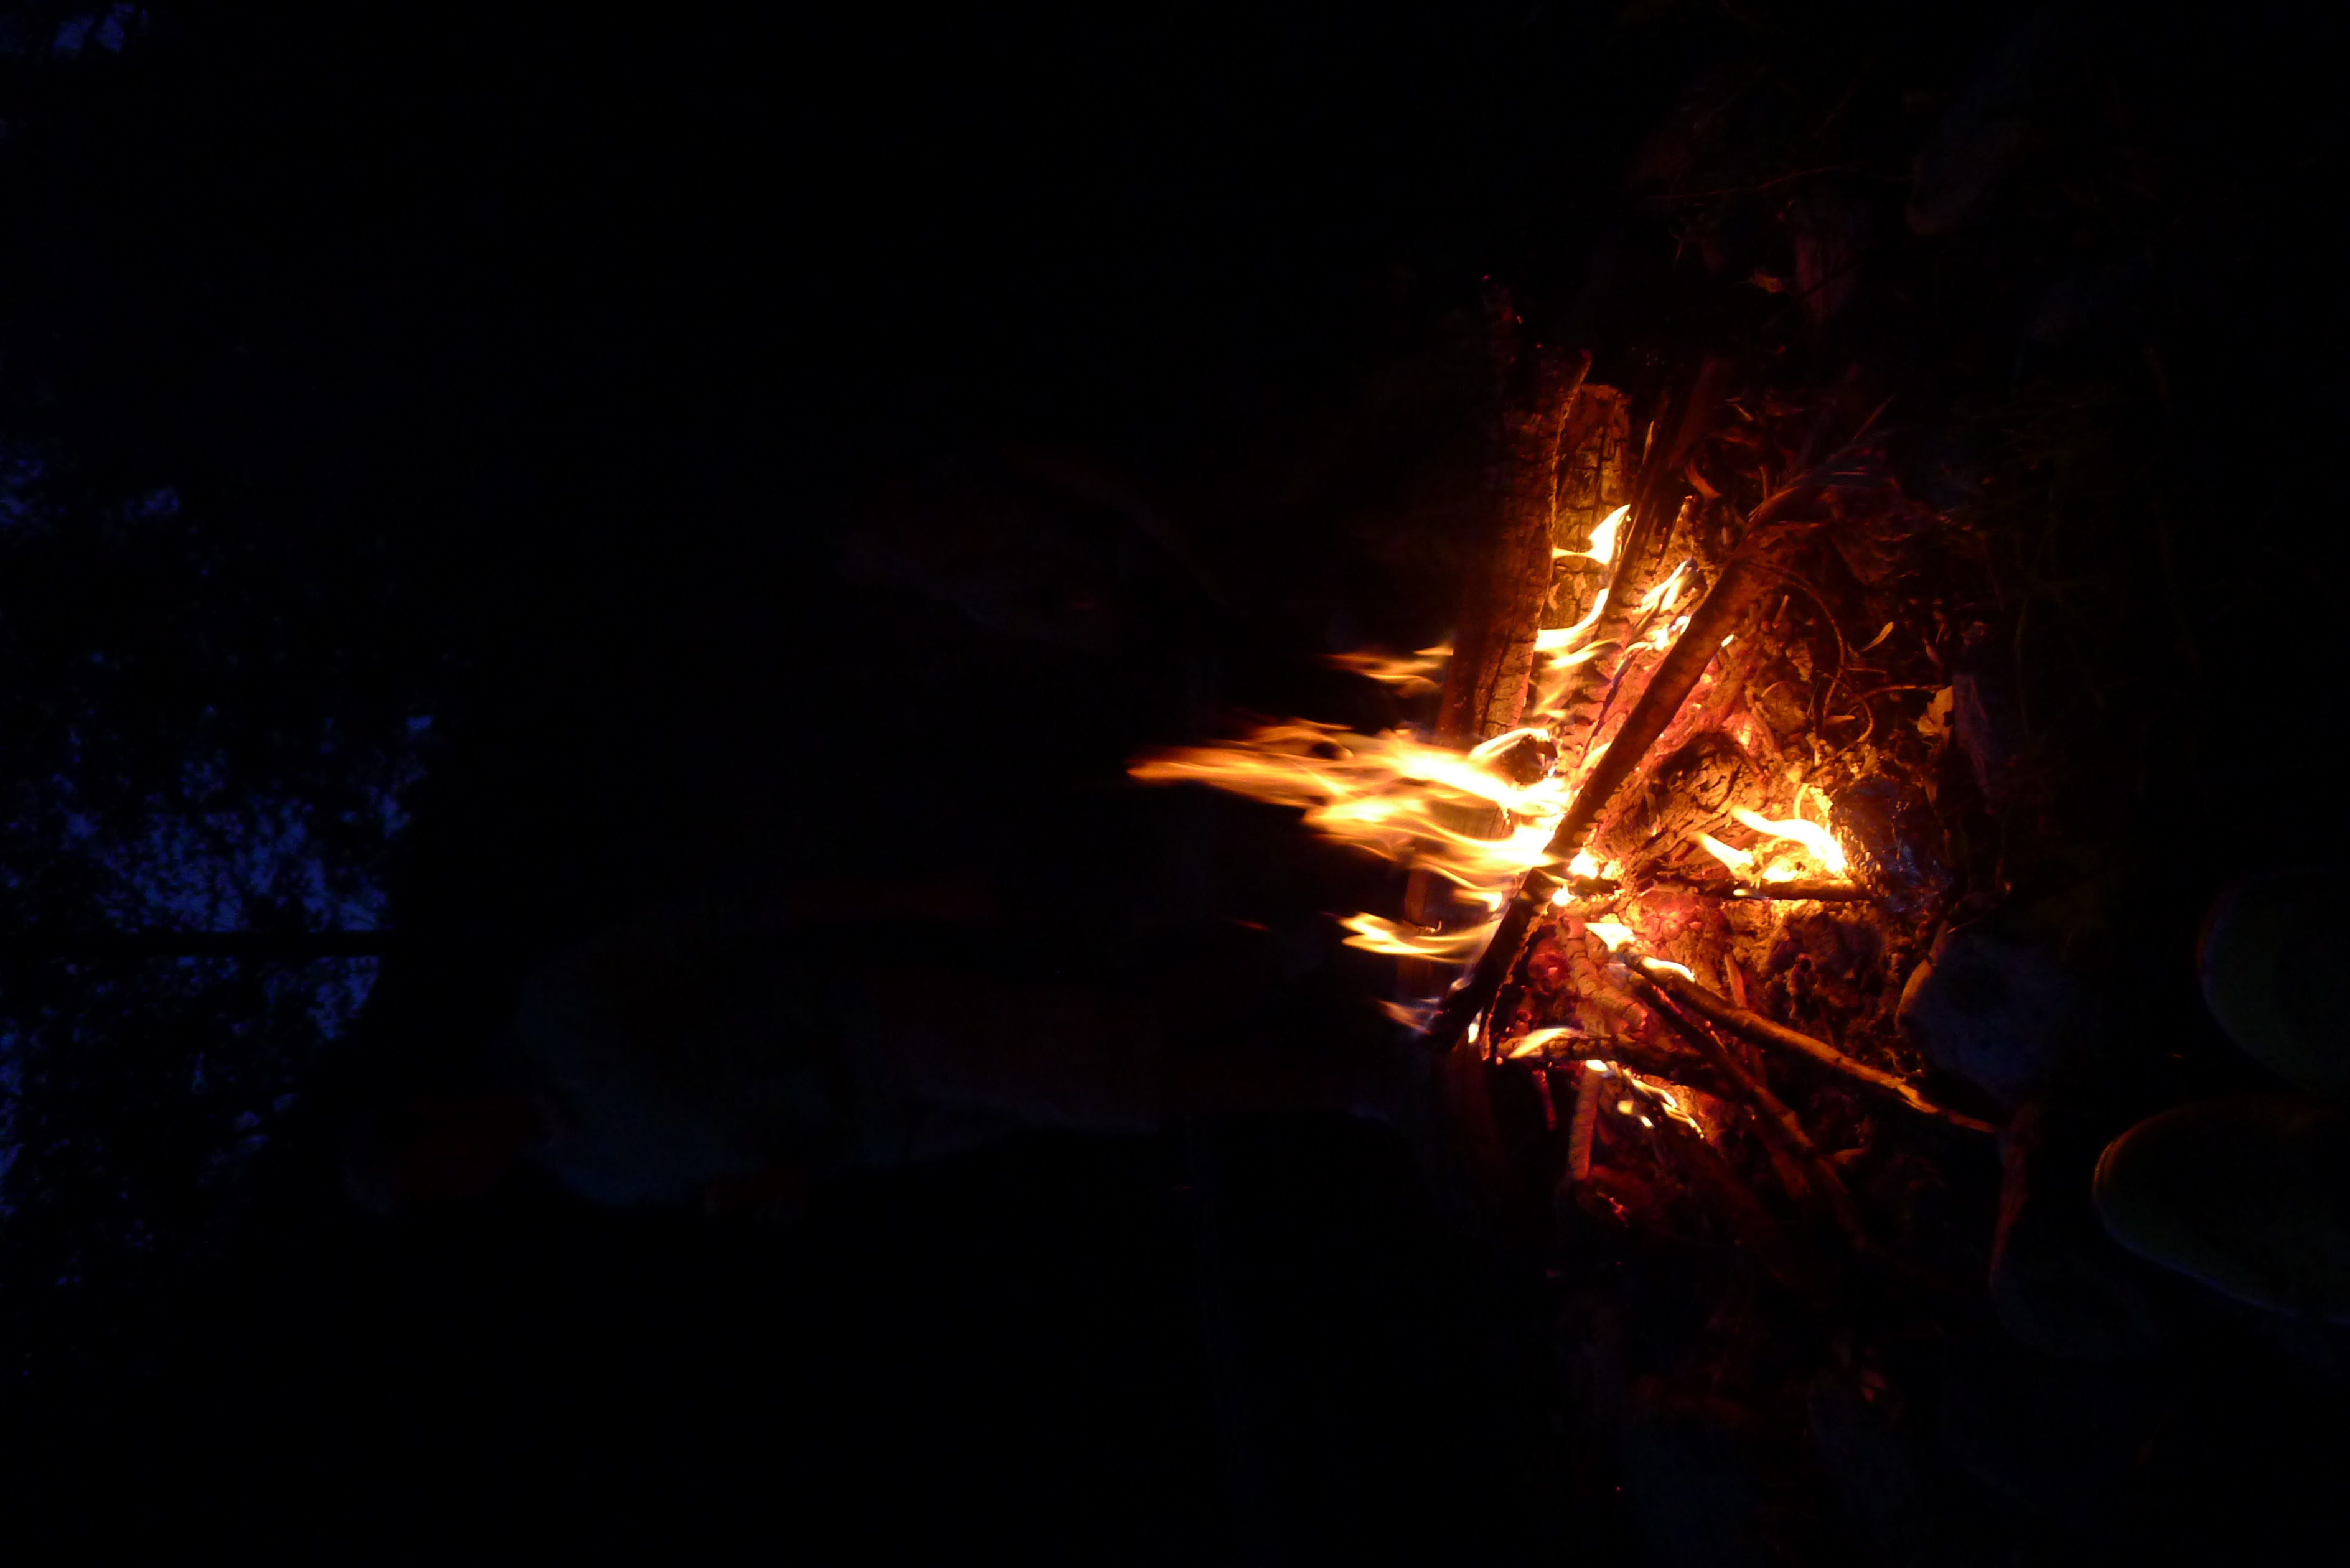
\includegraphics[width=.5\textwidth]{p1}
\\
Anmerkungen zu diesem Bild

\end{figure}

Text zwischen 2 Figures

\begin{figure}[!h]
\centering
\caption{Überschrift zu 2. Figure}
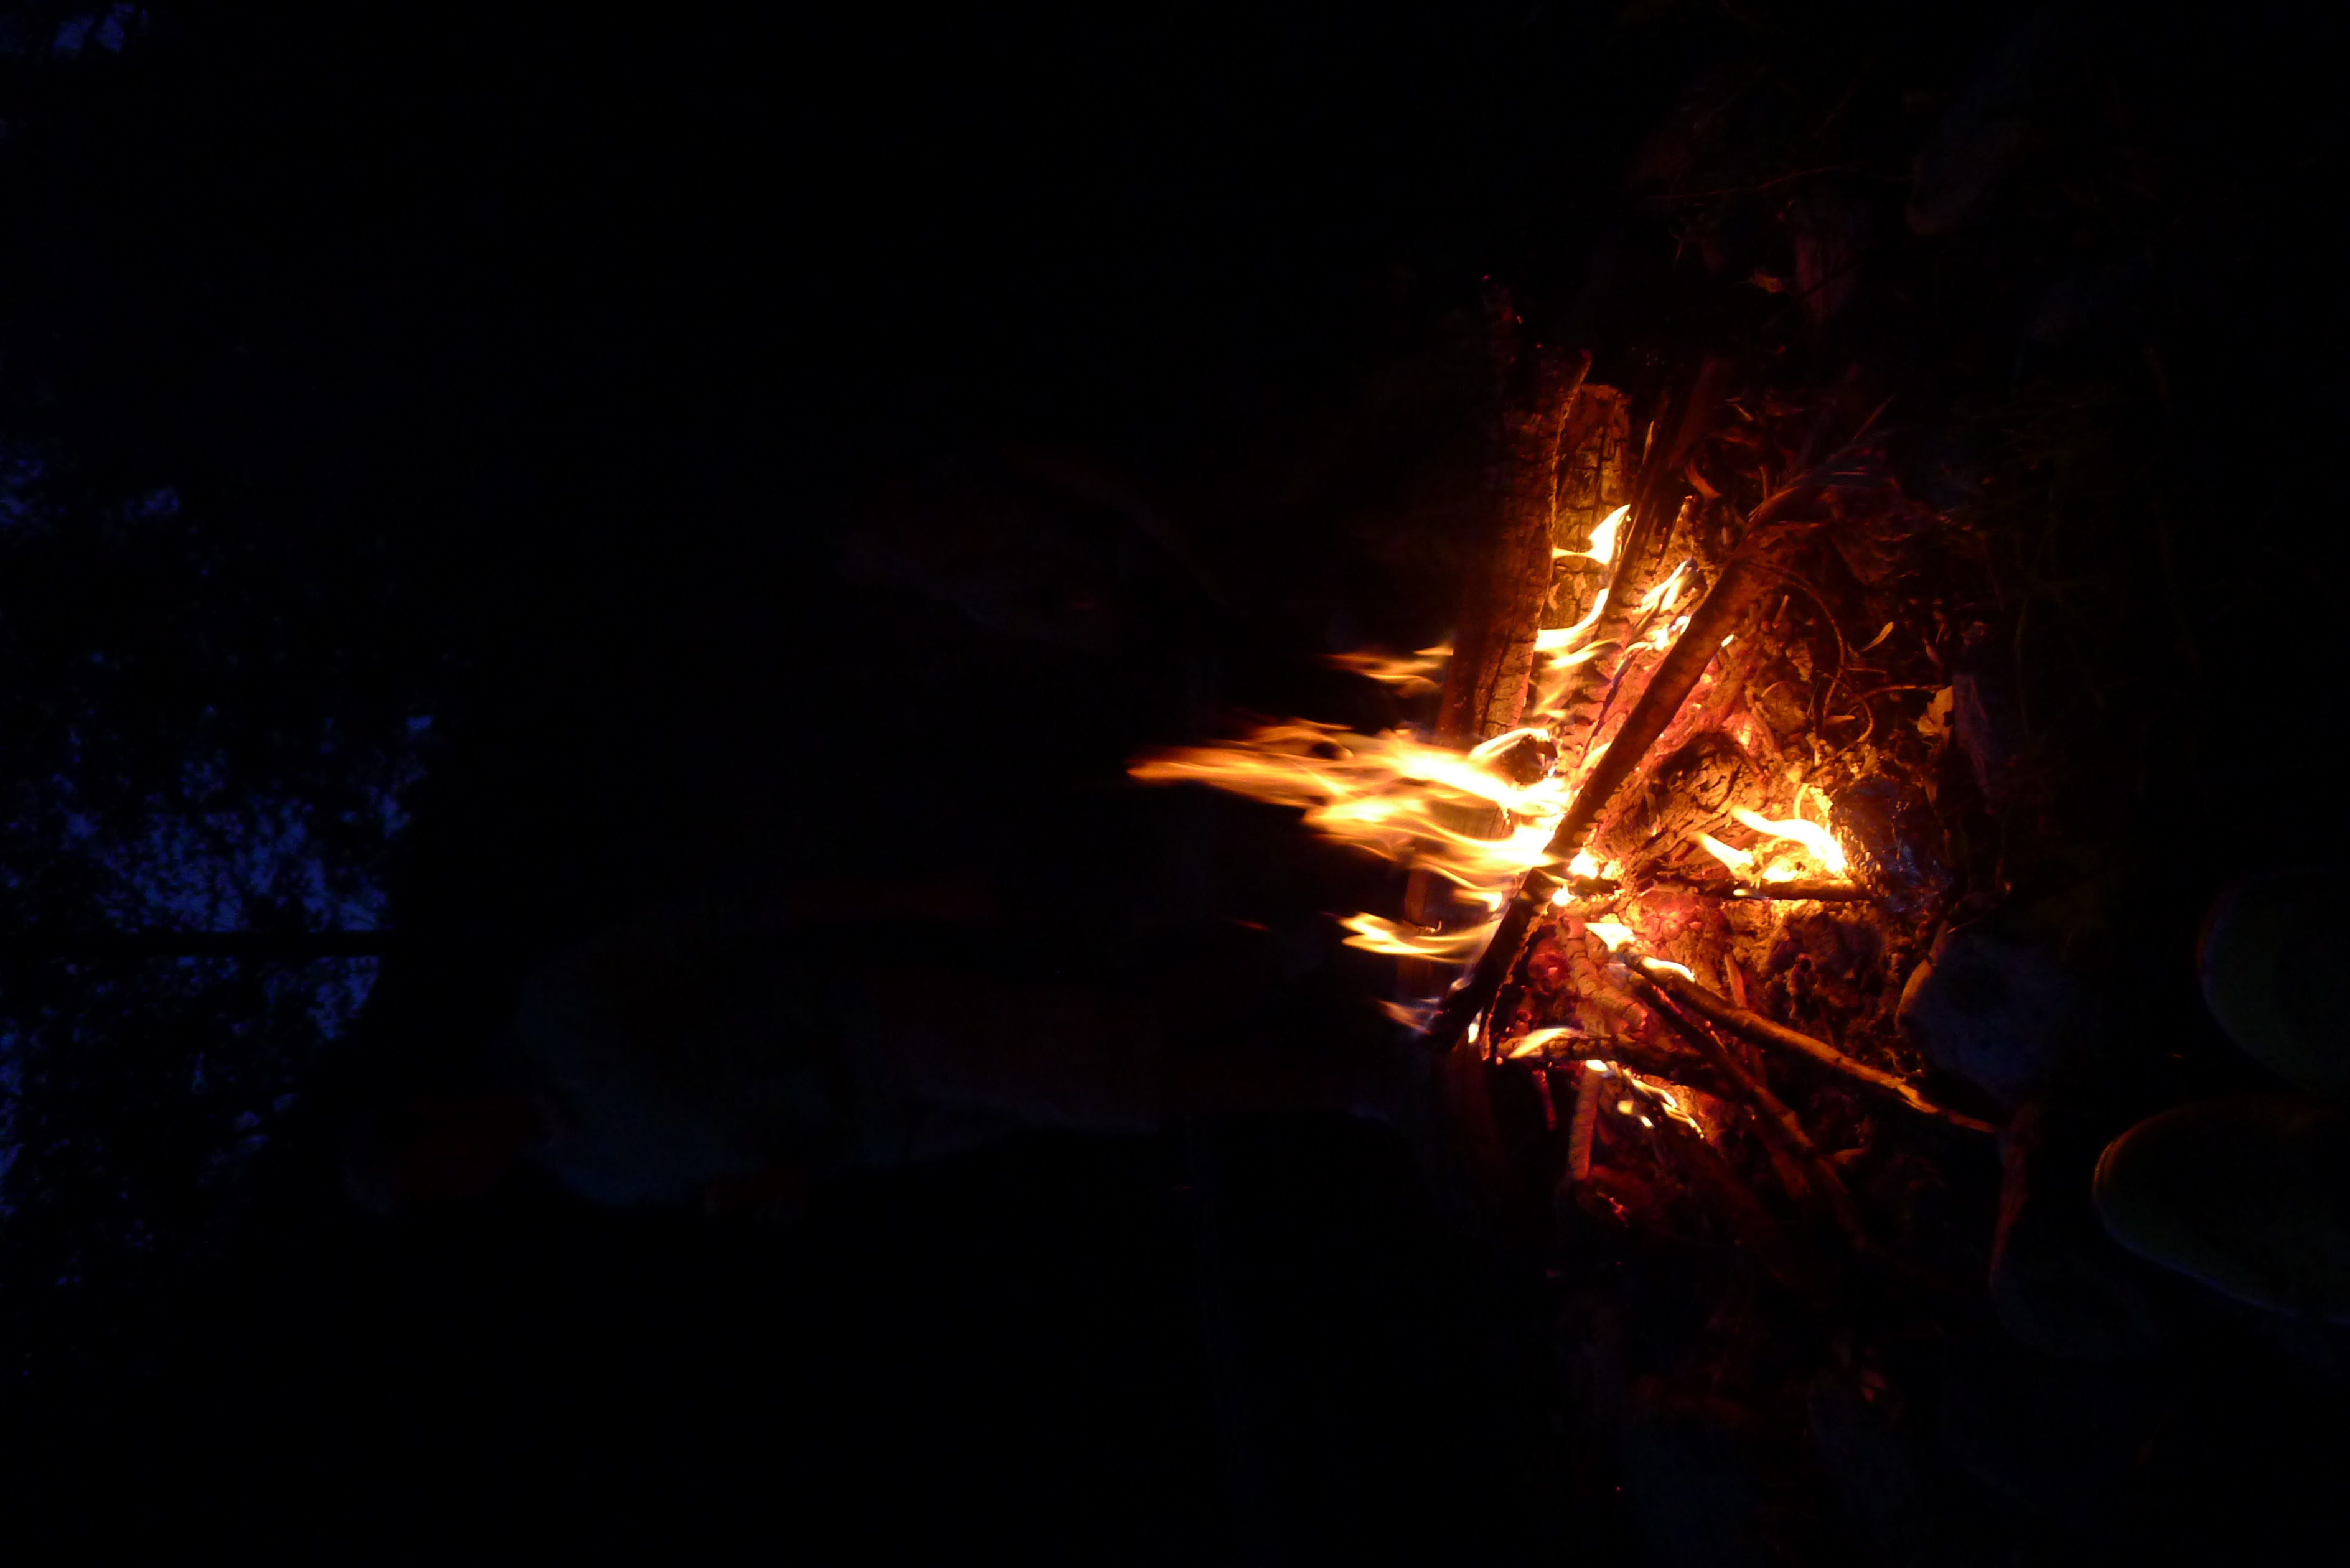
\includegraphics[height=\textwidth,angle=270]{p1}
\end{figure}

\clearpage
\section{Second section}
In this section\footnote{A section divides a report into several chapters, containing clearly distinct matter in a general content. Subsections however contain a more granular split of  common topic.}, we want to introduce footnotes, which are essential for the citation of sources. 

These footnotes\footnote{This is a footnote, for example.} show the use of the footnotes for \glqq citation\grqq{} purposes.
Dies ist \zb eine Abkürzung \vgl Hallodri hin oder her.



\noindent ein richtig greßer absatz
\subsection{subsection two}
\lipsum[2-2]
\subsection{subsection three}
\lipsum[3-3]
\subsection{Number four}
\lipsum[4-5]

\section{Just a section}
\lipsum[5-10]






\newpage
\pagestyle{empty}
%Bibliography
\section*{Literaturverzeichnis}
Göcke, M., Köhler, T. (2002), Außenwirtschaft – Ein Lern- und Übungsbuch, 1. Aufl., Heidelberg.

\bib{Autor, Vorname}{Jahr}{Titel}{Internetz}{\today}
\bib{Wikipedia}{o.J.}{Griechische Staatsshulden}{https://de.wikipedia.org}{\today}
Wikipedia Foundation Inc. (b), Griechische Staatsschuldenkrise, \url{https://de.wikipedia.org/wiki/Datei:GRSchuKrise.png}, 29.10.2015.




%Erklärung
\newpage
%*******************************************************
% Declaration
%*******************************************************
%\refstepcounter{dummy}
%\pdfbookmark[0]{Declaration}{declaration}
\section*{Erklärung}
\thispagestyle{empty}
\vspace{1cm}
Ich versichere hiermit, dass ich meine Master-Thesis
\vspace{1.5cm}\\
``\TitleGer''\\
 \vspace{1.5cm}\\
selbständig und ohne fremde Hilfe angefertigt habe und dass ich alle von anderen Autoren wörtlich übernommenen Stellen wie auch die sich an die Gedankengänge anderer Autoren eng anlehnenden Ausführungen meiner Arbeit besonders gekennzeichnet und die Quellen zitiert habe. Eine (durchsuchbare) digitale Fassung der Arbeit reiche ich ein und erlaube die Überprüfung mittels Anti-Plagiatssoftware. 


\vspace{2cm}
 
\noindent{Gießen, \myDate}

\vspace{2cm}

\begin{center}
    \begin{tabular}{m{5cm}}
        \\ \hline
        \centering\myName \\
    \end{tabular}
\end{center}
%Flushright
%Leere Seite
\newpage
\thispagestyle{empty}
\quad
\end{document}
